\subsection{Introduction}

\paragraph{} La résonance stochastique est un phénomène d'amplification de la réponse d'un système à un forçage périodique en présence de bruit. Ce qui caractérise cette résonance est que l'amplification est permise par le bruit agissant sur le système. Ceci est assez contre-intuitif, car généralement la présence de bruit à pour effet de couvrir la réponse au signal en se superposant à ce dernier.

\paragraph{} Un système élémentaire présentant un effet de résonance stochastique est celui constitué d'une particule dans un potentiel en double puits \cite{scholarpedia} -- voir figure \ref{fig:potentiel_double_puits}. La particule effectue naturellement des transitions d'un puits à l'autre à cause du bruit, mais lorsque le taux de ces transitions devient comparable à la fréquence du forçage externe, les transitions se synchronisent avec ce dernier -- voir figure \ref{fig:trajectory_resonant}. Ce phénomène amplifie drastiquement l'effet du forçage, malgré le fait qu'il soit trop petit pour conduire les transitions à lui seul.

\paragraph{} Une explication intuitive de ce mécanisme a été fournie par Benzi \cite{benzi2010} -- voir figure \ref{fig:explication_mecanisme}. L'idée est que le forçage décale périodiquement un puits du potentiel par rapport à l'autre, ce qui a pour effet de rendre les taux de transitions asymétriques et ainsi toujours maintenir la particule dans le puits favorisé par le forçage. 

\begin{figure}[t]
	\centering
	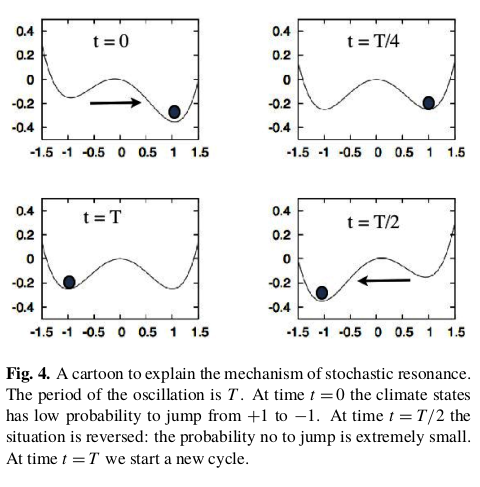
\includegraphics[width=0.8\linewidth]{figures/mecanisme_benzi_2010}
	\caption{Explication du mécanisme de résonance stochastique par R. Benzi. Image tirée de \cite{benzi2010}.}
	\label{fig:explication_mecanisme}
\end{figure}
